\chapter{Improving the Reliability of the Meteor Stegosystem}
\label{chap:reliability}

The Meteor authors have released an online demo of Meteor at \cite{MeteorDemo2021}.
On the website, they state that ``due to issues with the GPT-2 algorithm interface, you sometimes may see extra output from a decoded stegotext. This does not impact the underlying security of the scheme''.
After experimentation, we conclude that the cause of this is not due to issues with the algorithm interface but to the way GNNs with subword tokenization such as GPT-2 tokenize text.

In this chapter, we will, after describing the issue at hand, show that the Meteor Stegosystem is indeed unreliable by providing a counterexample.
Afterwards, we will discuss an experiment which approximates the probability of incorrect decodings.
The experiment shows that for sufficiently long hiddentexts the probability of incorrect decodings increases to approximately 87 \%.
To improve reliability, we present a change to Meteor's $Decode$ algorithm to increase the probability of successfully recovering the hiddentext message using a DFS-based graph search while -- in the worst case -- introducing computational overhead exponential in stegotext length.

\section{Ambiguous Tokenization}
\label{sec:amb-tok}

In \autoref{sec:generative-neural-networks}, we discussed that GNNs use a set of tokens to represent text.
To improve the quality of generated text, models (not only) in the GPT-n family use subword tokenization.
Subword tokenization is opposed to word tokenization, where text is split by spaces, and character based tokenization, where text is tokenized as a sequence of characters.
Subword tokenization allows for more effective machine learning, as the model can easier connect related words to each other.
This technique proved to be very effective in enhancing GNN performance in the last few years.

On the other hand, this allows for one word to have multiple tokenizations.
For example, the word ``doesn't'' might be tokenized as ``do$||$es$||$n't'', but it could also be tokenized as ``does$||$n't'' or even ``d$||$o$||$e$||$s$||$n$||$'$||$t''.
This situation is what we call an ambiguous tokenization.
If Alice generates a stegotext which has an ambiguous tokenization and Bob choses a different tokenization than Alice, the decoding will fail because a wrong prefix of the sample used to generate a token will be recovered from the stegotext.
For party $P \in \{A,B\}$ we denote by $T_P$ the tokenizer used to generate (encoding party $A$) or parse (decoding party $B$) a stegotext $c \in \Delta^*$ as a sequence of tokens $T_P(c) = t_1||t_2||\dots||t_{|t|} \in \mathcal{T}^*$.

To measure the difference in tokenizations of a given word between Alice and Bob, we define a distance function $D$ that measures the number of mismatching subsequences of two tokenizations $t,~ t'$ as follows:

\begin{definition}[Tokenization Distance]
Let $t = t_1 || t_2 || \dots || t_{|t|} \in \mathcal{T}^*,~ t' = t'_1 || t'_2 || \dots || t'_{|t'|} \in \mathcal{T}^*$ be sequences of tokens with $|t| \geq |t'|$ (otherwise, swap $t$ and $t'$).
If $t_1 \neq t'_1$ or $t_{|t|} \neq t'_{|t'|}$ prepend or append, respectively, the special empty token $\epsilon$ to both $t$ and $t'$.
Define the \emph{tokenization distance of $t$ and $t'$} as a function $D \colon \mathcal{T}^* \times \mathcal{T}^* \rightarrow \mathbb{N}$ with
$$D(t, t') = \big| \big\{ i \in [1, |t|-1] \mid \exists i' > 0 \exists l > 0 \exists l' \geq l: t_{i} = t'_{i'} \land \left( \bigwedge_{j=1}^{l} t_{i+j} \neq t'_{i'+j} \right) \land t_{i+l+1} = t'_{i'+l'+1} \big\} \big|.$$
\end{definition}

\begin{example}[Tokenization Distance]
Let $c = \textrm{``hello''}$ be a text generated by Alice with tokenization $T_A(c) = \textrm{he}||\textrm{l}||\textrm{lo}$.
Let $T_B(c) = \textrm{he}||\textrm{llo}$ be the tokenization of $c$ generated by Bob.
The distance between $T_A(c)$ and $T_B(c)$ is 

$$
D(T_A(c), T_B(c))
= D(\textrm{he}||\textrm{l}||\textrm{lo}, \textrm{he}||\textrm{llo})
= D(\textrm{he}||\textrm{l}||\textrm{lo}||\epsilon, \textrm{he}||\textrm{llo}||\epsilon)
= \left| \left\{ 1 \right\} \right| = 1.
$$
\end{example}

\section{Reliability of the Meteor Stegosystem}

In \autoref{alg:decode}, we see that during decoding, the stegotext $c$ generated by \autoref{alg:encode} should be parsed as $c = c_0 ||c_1 || \dots || c_{\tau}$.
This task is performed by a tokenizer over tokens $\mathcal{T}$.
Meteor's $Decode$ algorithm expects that the parsing of $c$ can recover the $c_i$ originally generated during encoding.
This unfortunately is, at least for models with subword tokenizations such as GPT-2, not the case for some combinations of hiddentext, key and history due to ambiguous tokenization described above.
In \autoref{sec:alg-rec-tok-candidates}, we will show how to fix these reliability issues.

\begin{theorem}
The Meteor stegosystem is not reliable.
\end{theorem}

\begin{proof}
For Meteor to be reliable, its unreliability must be negligible in $\lambda$, i.e.
$$UnRel_{\mathcal{S}}(\lambda) = \max_{\substack{k \in \{0,1\}^\lambda\\m \in \mathcal{U}^*\\ h \in \mathcal{H}}}\left\{ Pr[SD(k, SE(k,m,h), h) \neq m] \right\} < \mu(\lambda).$$ \todo{we removed $\mu$ from preliminaries}
We show unreliability by finding a tuple $(k',m',h')$ where decoding always fails, i.e. $$Pr[SD(k', SE(k',m',h'), h') \neq m] = 1.$$
The following counterexample has been generated by repeatedly encoding a fixed message $m'$ and history $h'$ with random keys $k' \leftarrowS U_{512}$.
We will later show that the decoding fails for many or most keys $k$, especially if the encoded messages $m$ are long ($|m| \geq 1024$ bytes).
Let

\begin{lstlisting}[breaklines]
k' = 0xb95e03a1d01b304f11dcf2bc844e5fd3cbed41253b0506876004207b2c2a10e
    2d89c1a40e93530bfcfaaee54e66ae048d2d2a536615b0a81afe792883877d5b6
m' = "Hello world"
h' = "Despite a long history of research and wide-spread applications to censorship resistant systems, practical steganographic systems capable of embedding messages into realistic communication distributions, like text, do not exist.\n\n"
\end{lstlisting}

The stegotext for these inputs when using the Meteor demo code at \cite{MeteorDemo2021} is

\begin{lstlisting}
c = '\nZeus communication system, controlled by anÆ2 desktop mic with'
\end{lstlisting}

When passed to the standard GPT-2 tokenizer, the substring ``Zeus'' of $c$ is parsed as ``Z$||$eus'', while the encoding party has generated ``Zeus'' with token sequence ``Ze$||$us''.
Therefore, the stegotext cannot be successfully decoded to the original hiddentext ``Hello world'', which violates reliability.
\end{proof}

After we have seen that this problem appears at least once by finding a counterexample, another question arises:
How often does this happen?
If this happens only for a negligible number of combinations of message, key, and history (or maybe even only for this exact combination), this might be a non-issue.

To approach this question, we first define a random variable $X$ as the distance between tokenizations $T_A(c)$ and $T_B(c)$ generated by Alice and Bob respectively for a stegotext $c \in \Delta^*$, i.e. for randomly chosen $c$ we define $X = D(T_A(c), T_B(c))$.

As we have argued in \autoref{sec:amb-tok}, the decoding can only succeed if no tokenization mismatches happen, i.e. the tokenizations generated by Alice and Bob respectively are the same.
Therefore, for a successful decoding of a stegotext, the tokenization distance must be zero.
We can establish the tokenization distance as an upper bound on the probability of a successful decoding:

$$Pr[Decode_{\mathcal{M}}^\beta(k, Encode_{\mathcal{M}}^\beta(k,m,h), h)=m] \leq Pr[X=0].$$

Unfortunately, we cannot determine $Pr[X=0]$ exactly because there are infinitely many stegotexts $c \in \Delta^*$.
Instead, we will estimate $Pr[X=0]$ with an experimentally determined approximation $\hat{Pr}_n[X=0]$ using samples $(k,m,h) \in S_n$ with keys $k \in \{0,1\}^\lambda$ for a fixed security parameter $\lambda$, messages $m \in M_n \subset \mathcal{U}^n$ for message lengths $n$ and histories $h \in \mathcal{H}$.
For every sample in $S_n$, we generate stegotexts $c = Encode_{\mathcal{M}}^\beta(k,m,h)$, determine the tokenization distances $D(T_A(c), T_B(c))$.
Afterwards, we can calculate the approximation
$$\hat{Pr}_n[X=0] = \frac{|\{ (k,m,h) \in S_n \mid D(T_A(Encode_{\mathcal{M}}^\beta(k,m,h)), T_B(Encode_{\mathcal{M}}^\beta(k,m,h))) = 0 \}|}{|S_n|}.$$

For the experiment, we used William Shakespeare's drama Hamlet as the source for messages and histories.
For the message set $M_n$, we used blocks of length $n=128$ and $1024$ bytes from the script of Hamlet, respectively.
The entire script of Hamlet is 191726 bytes long.
That gives us $|M_{128}|=\lceil \frac{191726}{128} \rceil = 1498$ and $|M_{1024}|= \lceil \frac{191726}{1024} \rceil = 188$ samples for $m$.
Even though the sample size for blocks of 1024 bytes is rather small, the average stegotext length grows proportionally to the number of bits encoded, so we can expect about the same total length of token sequences for both experiments.
For each hiddentext message, we generated a random key $k \leftarrowS U_{512}$ as well as an initial history $h$ of length 128 bytes randomly chosen from the script of Hamlet.

After we have defined the sample data, we encoded and subsequently decoded each sample using a modified version of the Meteor demo code from \cite{MeteorDemo2021}.
After decoding, we analyzed the tokens generated and computed the tokenization distances between Alice and Bob.

The experiment shows that most stegotexts have at least one mismatch if they are of significant length (\autoref{fig:meteor-stats-mismatch-count}).
When encoding 128 byte blocks, we get a success probability of $\hat{Pr}_{128}[X=0] \approx 0.57$.
When encoding larger blocks of 1024 bytes, it even decreases to $\hat{Pr}_{1024}[X=0] \approx 0.13$.

\begin{figure}[htbp]%
  \begin{subfigure}{.5\textwidth}%
    \centering%
      \resizebox{0.9\linewidth}{!}{%
      % This file was created with tikzplotlib v0.10.1.
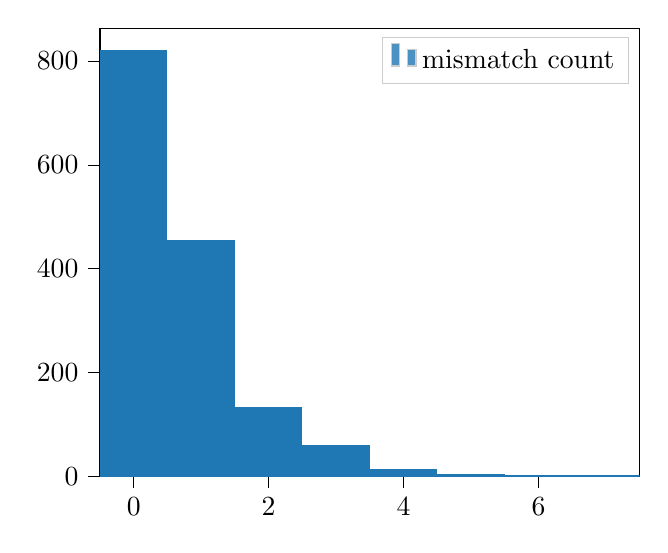
\begin{tikzpicture}

\definecolor{darkgray176}{RGB}{176,176,176}
\definecolor{lightgray204}{RGB}{204,204,204}
\definecolor{steelblue31119180}{RGB}{31,119,180}

\begin{axis}[
legend cell align={left},
legend style={fill opacity=0.8, draw opacity=1, text opacity=1, draw=lightgray204},
tick align=outside,
tick pos=left,
x grid style={darkgray176},
xmin=-0.5, xmax=7.5,
xtick style={color=black},
y grid style={darkgray176},
ymin=0, ymax=863.1,
ytick style={color=black}
]
\draw[draw=none,fill=steelblue31119180] (axis cs:-0.5,0) rectangle (axis cs:0.5,822);
\addlegendimage{ybar,ybar legend,draw=none,fill=steelblue31119180}
\addlegendentry{mismatch count}

\draw[draw=none,fill=steelblue31119180] (axis cs:0.5,0) rectangle (axis cs:1.5,455);
\draw[draw=none,fill=steelblue31119180] (axis cs:1.5,0) rectangle (axis cs:2.5,134);
\draw[draw=none,fill=steelblue31119180] (axis cs:2.5,0) rectangle (axis cs:3.5,61);
\draw[draw=none,fill=steelblue31119180] (axis cs:3.5,0) rectangle (axis cs:4.5,15);
\draw[draw=none,fill=steelblue31119180] (axis cs:4.5,0) rectangle (axis cs:5.5,5);
\draw[draw=none,fill=steelblue31119180] (axis cs:5.5,0) rectangle (axis cs:6.5,3);
\draw[draw=none,fill=steelblue31119180] (axis cs:6.5,0) rectangle (axis cs:7.5,3);
\end{axis}

\end{tikzpicture}
%
    }%
    \caption{128 bytes ($\hat{Pr}_{128}[X=0] = \frac{861}{1498} \approx 0.57$)}%
  \end{subfigure}%
  \begin{subfigure}{.5\textwidth}%
    \centering%
      \resizebox{0.9\linewidth}{!}{%
      % This file was created with tikzplotlib v0.10.1.
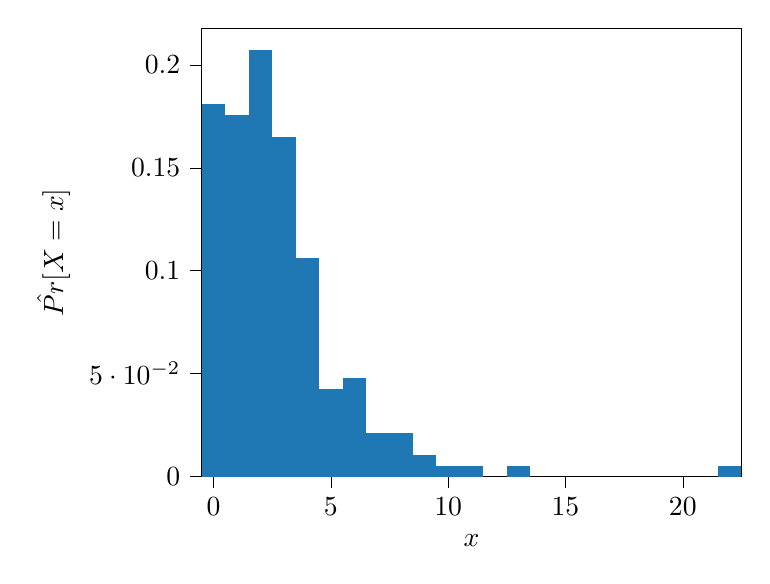
\begin{tikzpicture}

\definecolor{darkgray176}{RGB}{176,176,176}
\definecolor{steelblue31119180}{RGB}{31,119,180}

\begin{axis}[
tick align=outside,
tick pos=left,
x grid style={darkgray176},
xlabel={\(\displaystyle x\)},
xmin=-0.5, xmax=22.5,
xtick style={color=black},
y grid style={darkgray176},
ylabel={\(\displaystyle \hat{Pr}[X=x]\)},
ymin=0, ymax=0.21781914893617,
ytick style={color=black}
]
\draw[draw=none,fill=steelblue31119180] (axis cs:-0.5,0) rectangle (axis cs:0.5,0.180851063829787);
\draw[draw=none,fill=steelblue31119180] (axis cs:0.5,0) rectangle (axis cs:1.5,0.175531914893617);
\draw[draw=none,fill=steelblue31119180] (axis cs:1.5,0) rectangle (axis cs:2.5,0.207446808510638);
\draw[draw=none,fill=steelblue31119180] (axis cs:2.5,0) rectangle (axis cs:3.5,0.164893617021278);
\draw[draw=none,fill=steelblue31119180] (axis cs:3.5,0) rectangle (axis cs:4.5,0.106382978723405);
\draw[draw=none,fill=steelblue31119180] (axis cs:4.5,0) rectangle (axis cs:5.5,0.042553191489362);
\draw[draw=none,fill=steelblue31119180] (axis cs:5.5,0) rectangle (axis cs:6.5,0.0478723404255322);
\draw[draw=none,fill=steelblue31119180] (axis cs:6.5,0) rectangle (axis cs:7.5,0.021276595744681);
\draw[draw=none,fill=steelblue31119180] (axis cs:7.5,0) rectangle (axis cs:8.5,0.021276595744681);
\draw[draw=none,fill=steelblue31119180] (axis cs:8.5,0) rectangle (axis cs:9.5,0.0106382978723405);
\draw[draw=none,fill=steelblue31119180] (axis cs:9.5,0) rectangle (axis cs:10.5,0.00531914893617025);
\draw[draw=none,fill=steelblue31119180] (axis cs:10.5,0) rectangle (axis cs:11.5,0.00531914893617025);
\draw[draw=none,fill=steelblue31119180] (axis cs:11.5,0) rectangle (axis cs:12.5,0);
\draw[draw=none,fill=steelblue31119180] (axis cs:12.5,0) rectangle (axis cs:13.5,0.00531914893617025);
\draw[draw=none,fill=steelblue31119180] (axis cs:13.5,0) rectangle (axis cs:14.5,0);
\draw[draw=none,fill=steelblue31119180] (axis cs:14.5,0) rectangle (axis cs:15.5,0);
\draw[draw=none,fill=steelblue31119180] (axis cs:15.5,0) rectangle (axis cs:16.5,0);
\draw[draw=none,fill=steelblue31119180] (axis cs:16.5,0) rectangle (axis cs:17.5,0);
\draw[draw=none,fill=steelblue31119180] (axis cs:17.5,0) rectangle (axis cs:18.5,0);
\draw[draw=none,fill=steelblue31119180] (axis cs:18.5,0) rectangle (axis cs:19.5,0);
\draw[draw=none,fill=steelblue31119180] (axis cs:19.5,0) rectangle (axis cs:20.5,0);
\draw[draw=none,fill=steelblue31119180] (axis cs:20.5,0) rectangle (axis cs:21.5,0);
\draw[draw=none,fill=steelblue31119180] (axis cs:21.5,0) rectangle (axis cs:22.5,0.00531914893617025);
\end{axis}

\end{tikzpicture}
%
    }%
    \caption{1024 bytes ($\hat{Pr}_{128}[X=0] = \frac{25}{188} \approx 0.13$)}%
  \end{subfigure}%
  \caption{
  Tokenization mismatch count probability when using Meteor to encode Shakespeare's Hamlet block-wise for different block sizes.
  We denote the random variable $X$ as the number of encoding mismatches in a stegotext.
  The x-axis shows the number of tokenization mismatches between the encoding and the decoding party for hiddentext blocks of size...}
  \label{fig:meteor-stats-mismatch-count} 
\end{figure}

%In the same experiment, we have also measured the mismatch length, which is the number of tokens which have to be skipped in the stegotext to get back in sync with the decoding party.
%For example, if a stegotext ``steganography is great'' was encoded with token sequence (steg, ano, graphy, \verbvisiblespace is, \verbvisiblespace great), but decoded as (ste, ga, no, graphy, \verbvisiblespace is, \verbvisiblespace great), the mismatch length is two, because the two tokens \emph{steg} and \emph{ano} have to be skipped on the encoded token sequence to get back in sync between encoding and decoding party when encounterint the token \emph{graphy}
%This measure will later help us estimate how far we should look ahead in the stegotext when trying to recover from decoding errors.

%\begin{figure}[htbp]%
% \begin{subfigure}{.5\textwidth}%
%   \centering%
%     \resizebox{0.8\linewidth}{!}{%
%     \input{fig_meteor_stats_mismatch_length_128.tikz}%
%   }%
%   \caption{128 bytes}%
% \end{subfigure}%
% \begin{subfigure}{.5\textwidth}%
%   \centering%
%     \resizebox{0.8\linewidth}{!}{%
%     \input{fig_meteor_stats_mismatch_length_1024.tikz}%
%   }%
%   \caption{1024 bytes}%
% \end{subfigure}%
% \caption{
% Token mismatch length statistics when using Meteor to encode Shakespear's Hamlet blockwise for different block sizes.
% The x-axis shows the lengths of tokenization mismatches of the decoding party for hiddentext blocks of size...}
% \label{fig:meteor-stats-mismatch-count} 
%\end{figure}

Therefore, we have to find a way to deal with these failed decodings, especially if we plan to encode hiddentext of significant length such as HTTP messages or Diffie-Hellman key exchange messages.
In \autoref{sec:alg-rec-tok-candidates}, we will present an approach to recover from decoding errors while -- in the worst case and for some models -- introducing computational overhead exponential in stegotext length. 
In \autoref{chap:twowaycommunication}, we will show how we can split the hiddentext message and use DialoGPT -- a derivation of GPT-2 -- to generate chat-like stegotext.
Splitting the hiddentext results in shorter stegotext and thus decreases the probability of tokenization mismatches.



\section{Algorithmic Reconstruction of Token Candidates}
\label{sec:alg-rec-tok-candidates}

Unfortunately, with subword tokenization, the decoding party cannot decide which tokens have been used to generate a given stegotext.
To allow successful decoding of ambiguously tokenized stegotexts, we will introduce modifications to the $Encode$ and $Decode$ algorithms to detect and fix wrong tokenizations.

Before encoding, split the message $m$ into blocks $m_i$ of length $\gamma$.
After each block $m_i$, add a checksum block $q_i = q(m_i)$ of length $\delta$ into the hiddentext, i.e. $q \colon \{ 0,1 \}^\gamma \rightarrow \{ 0,1 \}^\delta$.
This value helps the decoder to decide if the decoding is still correct up to the block $i$.
By adding checksum blocks, we introduce $\delta \cdot \frac{|m|}{\gamma}$ bits of overhead to the hiddentext.
For the modified $MarkedEncode$ algorithm, see \autoref{alg:marked-encode}.

Now the decoding party Bob has to verify that after each block $m_i$ of $\gamma$ bits, the checksum $q(m_i)$ of length $\delta$ appears.
If not, a decoding error has occured in the stegotext, i.e. a tokenization mismatch has been occured.
To recover from this, Bob has to roll back his decoding and generate all possible tokenizations of a substring of $c$ starting with the position in $c$ after his last successful checksum check.
The BPE tokenizer used in GPT-2 does not contain tokens that span word boundaries, i.e. no token contains inner spaces. Therefore, we can assume that a tokenization mismatch ends when the current word does.
When a tokenization with correct checksums was found, the decoder expects that the correct tokenization has been found and proceeds.
Note that this approach will not work with models that use language independent tokenizers such as SentencePiece \cite{SentencePiece2018}, which tokenize strings as raw sentences and treats spaces as regular characters.
With language independent tokenizers, the entire suffix of $c$ starting with the block failing the checksum has to be considered, potentially introducing overhead exponential in stegotext length.

It is still possible that a wrong tokenization randomly yields a correct checksum.
In an actual implementation, one might want to check multiple blocks in advance before expecting that the correct tokenization has been found and/or choose $\gamma$ and $\delta$ depending on the security parameter $\lambda$ such that the probability of a false-positive checksum is negligible.
Determining specific values for $\gamma$ and $\delta$ is a trade-off between stegotext length and computational overhead in the case of a decoding error.
While longer checksums $\delta$ potentially decrease the risk of false-positive checksum checks, longer checksums cause longer stegotexts.
If we chose $\gamma = |m|$, only one checksum is generated over the entire message. 
If an error is detected after decoding the entire hiddentext, every possible tokenization for the stegotext $c$ has to be generated, of which there are exponentially many in stegotext length.
If we choose a small $\gamma$, many checksums are inserted, drastically increasing stegotext length.
A modified $Decode$ algorithm can be found in \autoref{alg:marked-decode}.

\begin{Pseudocode}[caption={
$MarkedEncode$ algorithm.
The modification this algorithm introduces is that after every block $m_i$ of $\gamma$ bits a checksum $q(m_i)$ is inserted into the hiddentext.
This allows the recipient to check for decoding errors after decryption.
$q$ is a function $q \colon \{0,1\}^\gamma \rightarrow \{0,1\}^\delta$ which generates a checksum of length $\delta$ for a message block of length $\gamma$.
}, label={alg:marked-encode}]
algorithm $MarkedEncode_{\mathcal{M}}^{\beta, \gamma, \delta}(k_{prg}, m, h, q)$
  Output: Stegotext message $c$
  $c \leftarrow \epsilon,~ n \leftarrow 0,~ i \leftarrow 0$
  Parse $m$ as blocks $m_1||m_2||\dots||m_\xi$ of size $\gamma$
  $m^* \leftarrow m_1||q(m_1)||m_2||q(m_2)||\dots||m_\xi||q(m_\xi)$
  while $n < |m^*|$ do
    $mask \leftarrow PRG.Next(k_{prg})$
    $r \leftarrow m^*[n:n+\beta] \oplus mask$
    $c_i \leftarrow Sample_{\mathcal{M}}^\beta(h, r)$
    $\mathcal{R} = Recover_{\mathcal{M}}^\beta(h, c_i)$
    $n_i \leftarrow LenPrefix^\beta(\mathcal{R})$
    $c \leftarrow c || c_i, n \leftarrow n+n_i, h \leftarrow h||c_i,~ i \leftarrow i + 1$
  Output $c$
\end{Pseudocode}

\begin{Pseudocode}[caption={
$MarkedDecode$ algorithm.
In comparison to Meteor's $Decode$ algorithm, $MarkedDecode$ verifies the checksums $q(m_i)$ of blocks $m_i$.
If the checksum does not match, a decoding error occured.
It then performs a lookbehind on the stegotext and generates all possible tokenizations $paths$ for a substring of $c$.
Afterwards, rewind the internal state and retry decoding with a path $p$ selected from $paths$.
}, label={alg:marked-decode}]
algorithm $MarkedDecode_{\mathcal{M}}^{\beta,\gamma,\delta}(k_{prg}, c, h, q)$
  Output: Plaintext message $m$
  $m^* \leftarrow \epsilon,~ n \leftarrow 0,~ j \leftarrow 0,~ \alpha^* \leftarrow 0$
  $paths \leftarrow \emptyset$
  Parse $c$ as $c_0 || c_1 || \dots || c_{\tau}$
  for $i \in \{ 0, 1, \dots, \tau \}$ do
    $\mathcal{R} = Recover_{\mathcal{M}}^\beta(h, c_i)$
    $n_i \leftarrow LenPrefix^\beta(\mathcal{R})$
    $n \leftarrow n + n_i$
    $j \leftarrow j + n_i$
    $m_i \leftarrow Prefix^\beta(\mathcal{R})$
    $mask \leftarrow PRG.Next(k_{prg})$
    $m^* \leftarrow m^* || (m_i \oplus mask[0: |m_i|])$
    $h \leftarrow h||c_i$
    if $j \geq \gamma + \delta$
      # calculate checksum
      Parse $m^*$ as $m^*_1||q_1||m^*_2||q_2||\dots||m^*_{\alpha^*}||q_{\alpha^*}||\dots||m^*_\alpha||q_\alpha$ ignoring suffix of length $< \gamma+\delta$
      if $q_{\alpha^*+1} \neq q(m^*_{\alpha^*+1}) \lor q_{\alpha^*+2} \neq q(m^*_{\alpha^*+2}) \lor \dots \lor q_\alpha \neq q(m^*_\alpha)$
        Find first index $j^* > i^*$ such that $c_{j^*}$ starts with space
        $c^* \leftarrow c_{i^*} || c_{i^*+1} || \dots || c_{j^*-1}$
        if $paths = \emptyset$
          $paths \leftarrow AllPaths(TokenizeCandidates_{\mathcal{T}}(c^*), c^*)$
        $p \leftarrow SelectPath(paths)$
        $paths \leftarrow paths~ \backslash~ p$
        replace $c_{i^*}||c_{i^*+1}||\dots||c_{j^*-1}$ in $c$ with $p$
        rewind PRG state and variables to state at $i^*$
        retry decoding starting with $m_{\alpha^*+1}$ with $p$
      else  # checksum verified, expect first $\alpha$ blocks and $i$ tokens to be correctly decoded
        $j \leftarrow j \mod (\gamma+\delta)$
        $paths \leftarrow \emptyset$
        $\alpha^* \leftarrow \alpha$
        $i^* \leftarrow i$
  Parse $m^*$ as $m^*_1||q(m^*_1)||m^*_2||q(m^*_2)||\dots||m^*_\xi||q(m^*_\xi)$
  Output $m \leftarrow m^*_1||m^*_2||\dots||m^*_\xi$
\end{Pseudocode}

For the modifications in $MarkedDecode$, we need helper algorithms $TokenizeCandidates_{\mathcal{T}}$, $AllPaths$ and $SelectPath$.

$TokenizeCandidates_{\mathcal{T}}$ generates a graph that represents the possible tokenizations of a given stegotext.
When passed a string $c$, the algorithm $TokenizeCandidates$ generates a directed, acyclic graph (or DAG) $G = (V, E)$.
The nodes $V$ represent all reachable suffix strings of $c$ (including the empty string $\epsilon$) using tokens from $\mathcal{T}$ with $|V| \leq |c| + 1$.
Edges $E$ represent tokens used to transition between suffixes.
For an example graph for input ``hello'', see \autoref{fig:ex-graph-tokenize-candidates}.
For example, ``hello'' can be transformed to ``lo'' with token ``hel''.

$AllPaths$ takes a graph $G = (V, E)$ generated by $TokenizeCandidates_{\mathcal{T}}(c)$ for a stegotext $c$ and a start node $v_i \in V$ as inputs and returns a set of all possible paths between $v_i$ and a fixed sink $v_j = \epsilon$ (the empty suffix).
Each path in that list represents a possible tokenization of $c$.
But how many paths exist between $v_i$ and $v_j$?
A path between two vertices is a set $V' \subseteq V$ that contains both $v_i$ and $v_j$ where there exist edges in $E$ from topologically greater vertices to topologically smaller vertices in $V'$.
In a complete DAG, there are up to $2^{|V|-2} \leq 2^{|c|-1}$ subsets of $V$ which contain both $v_i$ and $v_j$.
Therefore, the output size of $AllPaths$ is, in the worst case, exponential in input length.
For a DFS-based implementation of $AllPaths$ see \autoref{alg:all-paths}.

Lastly, $SelectPath$ selects a path from a list of $paths$ generated by $AllPaths$.
A simple strategy is to choose one element at random and try to decode it.
With this approach, we will find the correct tokenization on average after $\frac{|paths|}{2} \leq \frac{2^{|c|-1}}{2} = 2^{|c|-2}$ attempts.
While there are more advanced strategies to select a tokenization, e.g. by selecting a tokenization according to the probability distribution generated by the ML model, this simple approach is still viable when using the english language since we only generate paths for single words that are relatively short.
As has been shown by analyzing books from different epochs, the average word length in the english language is about five characters \cite{BoShSo2012}.
Therefore, an average english word can have up to $2^4 = 16$ possible tokenizations.
There still are commonly used (and therefore generated) words with a length of up to 13 characters such as ``international'' or ``circumstances'', which could have up to $2^{12} = 4096$ possible tokenizations.
Our experiments have shown that when using the GPT-2 tokenizer, the graphs for common longer words of the english language are still relatively small with less than $2^{11}$ possible paths.
For an implementation of $SelectPath$ that chooses a path at random see \autoref{alg:select-path-rnd}.



\begin{Pseudocode}[float,caption={
$TokenizeCandidates$ algorithm.
This generates a graph $G = (V, E)$ from a string $c$.
Vertices are substrings of $c$, each edge represents a token to use to transform between substrings.
This algorithm can be sped up by using dynamic programming to cache results of invocations of $TokenizeCandidates$.
}, label={alg:tokenize-candidates}]
algorithm $TokenizeCandidates_{\mathcal{T}}(c)$
  Output: Graph $G = (V, E)$
  if $c = \epsilon$
    return $(\emptyset, \emptyset)$
  for $t \in \{ t' \in \mathcal{T}~ |~ t' \textrm{ is prefix of } c \}$ do
    $V \leftarrow V \cup \{ c[|t|{:}] \}$
    $E \leftarrow E \cup \{ (c, c[|t|{:}]) \}$
    $G \leftarrow G \cup TokenizeCandidates_{\mathcal{T}}(c[|t|{:}])$
  return $G$
\end{Pseudocode}

\begin{figure}[htbp]
  \centering
  \begin{tikzpicture}
    \node[block] (hello) {hello};
    \node[block, right=15mm of hello] (lo) {lo};
    \node[block, above=15mm of lo] (llo) {llo};
    \node[block, above=15mm of llo] (ello) {ello};
    \node[block, below=15mm of lo] (o) {o};
    \node[block, right=15mm of lo] (bot) {$\epsilon$};
    
    \draw[->] (hello) to node[above] {h} (ello);
    \draw[->] (hello) to node[above] {he} (llo);
    \draw[->] (hello) to node[above] {hel} (lo);
    \draw[->] (hello) to node[left] {hell} (o);
    \draw[->, bend right=90,looseness=2] (hello) to node[below] {hello} (bot);

    \draw[->] (ello) to node[right] {e} (llo);
    %\draw[->, bend left=30] (ello) to node[right] {el} (lo);
    %\draw[->, bend left=30] (ello) to node[above] {ell} (o);
    \draw[->] (ello) to node[right] {ello} (bot);

    \draw[->] (llo) to node[right] {l} (lo);
    %\draw[->, bend right=30] (llo) to node[above] {ll} (o);
    %\draw[->] (llo)   to node[above] {llo} (bot);

    \draw[->] (lo)    to node[right] {l} (o);
    \draw[->] (lo)    to node[above] {lo} (bot);

    \draw[->] (o)     to node[above] {o} (bot);
  \end{tikzpicture}
  \caption{
Tokenization graph generated by $TokenizeCandidates_{\mathcal{T}}(\textrm{``hello''})$ with tokens $\mathcal{T} = \{ h, e, l, o, he, lo,  hel, hell, ello, hello \}$.
The vertices represent substrings of $c = \textrm{``hello''}$ which are accessible by removing a prefix token $t \in \mathcal{T}$ from $c$.
The edges are labeled with the token $t \in \mathcal{T}$ used to transform the left-hand side vertex $v_i$ to the right-hand side vertex $v_j$, i.e. $v_i = t || v_j$.
The special node $\epsilon$ represents the empty string and is a sink in the tokenization graph.
The list of all possible paths between $c$ and $\epsilon$ are the possible tokenizations of $c$ using tokens $\mathcal{T}$.
}
  \label{fig:ex-graph-tokenize-candidates}
\end{figure}

\begin{Pseudocode}[float,caption={
DFS-based $AllPaths$ algorithm that generates a list of all possible paths between between a root and a sink $\epsilon$ in a DAG.
This algorithm's performance can be sped up by using dynamic programming to cache results of invocations of $AllPaths$.
},label={alg:all-paths}]
algorithm $AllPaths(G, root)  $
  Output: List of paths between $root$ and sink $\epsilon$
  if $root = \epsilon$ do
    return $\epsilon$
  $paths \leftarrow \emptyset$
  $hops \leftarrow OutEdges(G, root)$
  for $hop \in hops$ do
    $subpaths \leftarrow AllPaths(G, hop, sink)$
    for $subpath \in subpaths$ do
      $paths \leftarrow paths \cup \{ root || subpath \}$
  return $paths$
\end{Pseudocode}

\begin{Pseudocode}[float, caption={
$SelectPath$ algorithm with random path selection strategy.
}, label={alg:select-path-rnd}]
algorithm $SelectPath(paths = \{ p_1, p_2, \dots, p_{|paths|} \})$
  Output: path $p \in paths$
  $i \leftarrowS \{1, 2, \dots, |paths| \}$
  $paths \leftarrow paths \backslash \{ p_i \}$
  return $p_i$
\end{Pseudocode}

%\begin{Pseudocode}[float, caption={
%Probabilistic Path Selection Strategy.
%}, label={alg:select-path-prob}]
%algorithm $SelectPath_{\mathcal{M}}(paths = \{ p_0, p_1, \dots, p_{|paths|-1} \}, h)$
% Output: path $p \in paths$
% $\mathcal{T}, \mathcal{P} \leftarrow Next_{\mathcal{M}}(h)$
% $p_i \leftarrow p_i \in paths$ such that $p_i$ starts with $t_j \in \mathcal{T}$ and $x_j \in \mathcal{P} = %max(\mathcal{P})$
  %$paths \leftarrow paths - \{ p_i \}$
  %return $p_i$
%\end{Pseudocode}
